\documentclass[12pt,letterpaper]{article}
\usepackage[latin1]{inputenc}
\usepackage[spanish]{babel}
\usepackage{graphicx}
\usepackage[left=2cm,right=2cm,top=2cm,bottom=2cm]{geometry}
\usepackage{graphicx} % figuras
\usepackage{subfigure} % subfiguras
\usepackage{float} % para usar [H]
\usepackage{amsmath}
\usepackage{txfonts}
\usepackage{stackrel} 
\usepackage[latin1]{inputenc}
\usepackage{multirow}
\usepackage{enumerate} % enumerados
\renewcommand{\labelitemi}{$-$}
\renewcommand{\labelitemii}{$\cdot$}
\author{Nelia Escalante}
\title{Caratula}
\begin{document}


\author{Nelia Escalante}
\title{Caratula}

\begin{titlepage}
\begin{center}
\large{UNIVERSIDAD PRIVADA DE TACNA}\\
\vspace*{-0.025in}
\begin{figure}[htb]
\begin{center}

\includegraphics[width=8cm]{./IMG/logo}
\end{center}
\end{figure}
\vspace*{0.15in}
INGENIERIA DE SISTEMAS  \\

\vspace*{0.5in}
\begin{large}
TITULO:\\
\end{large}

\vspace*{0.1in}
\begin{Large}
\textbf{RESULTADO DEL LABORATORIO 01} \\
\end{Large}

\vspace*{0.3in}
\begin{Large}
\textbf{CURSO:} \\
\end{Large}

\vspace*{0.1in}
\begin{large}
INTELIGENCIA DE NEGOCIOS\\
\end{large}

\vspace*{0.3in}
\begin{Large}
\textbf{DOCENTE:} \\
\end{Large}

\vspace*{0.1in}
\begin{large}
 Ing. Patrick Cuadros Quiroga\\
\end{large}

\vspace*{0.2in}
\vspace*{0.1in}
\begin{large}
ESTUDIANTE: \\
\begin{flushleft}
Escalante Maron, Nelia 		\hfill	(2014049551) \\

\end{flushleft}
\end{large}
\end{center}

\end{titlepage}


 \tableofcontents
 \newpage

 
\section{Desarrollo} 
LABORATORIO 01\\

Crear un reporte asociado a los datos de negocio\\
Basado en el conjunto de datos "credit data.csv"\\

Crear un reporte con la siguiente descripci\'on:\\

- Periodo de analisis: de 2014 a 2015\\
- Unidad de Tiempo: Trimestral (y total anual)\\
- Grupos de analisis: Por ingreso mensual con grupos.\\
	- menos de 2.500\\
	- 2.500 a 5.000\\
	- 5.000 a 10.000\\
	- mas de 10.000\\
- KPIs:\\
	- N\'umero de Cr\'editos\\
	- delincuencia promedio (porcentaje de clientes en morosidad de 90dpd) ingreso mensual promedio\\
- Estructura de tabla:\\
	- cuartos en columnas\\
	- Grupos y KPIs en filas.\\
- Dibuja una gr\'afica con:\\
	- Barras apiladas para el n\'umero de cr\'editos\\
	- L\'ineas para la morosidad media\\
Adicional, Analisis de Data Exploratorio:\\

- Crear un par gr\'afico de parejas para todas las variables\\
- Crear un gr\'afico con Ingresos VS Edad en el medio, m\'as distribuciones marginales\\

- Importar Informacion\\

Antes de comenzar tenemos que importar el archivo excel\\
\begin{center}
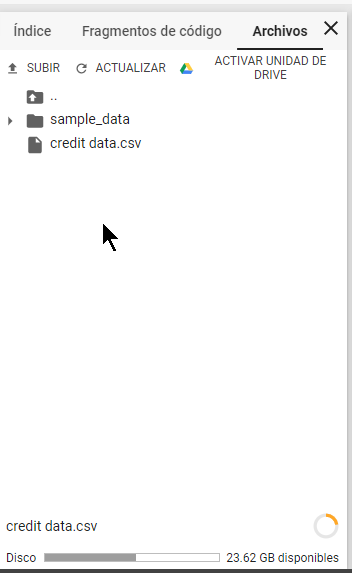
\includegraphics[width=9cm]{IMG/1.png} 
\end{center}


Importamos librerias y las describimos a continuacion:\\
- numpy: NumPy es una extensi\'on de Python, que le agrega mayor soporte para vectores y matrices, constituyendo una biblioteca de funciones matem\'aticas de alto nivel para operar con esos vectores o matrices.\\
- pandas: pandas es una API de an\'alisis de datos en columnas, ideal para manipular y analizar datos de entrada. Adem\'as, muchos marcos de trabajo de AA admiten las estructuras de datos pandas como entradas. Si bien una introducci\'on detallada a la API de pandas abarcar\'ia muchas p\'aginas, los conceptos principales que presentamos a continuaci\'on son simples. Para obtener una referencia m\'as completa, el sitio de documentaci\'on de pandas incluye una documentaci\'on exhaustiva y numerosos instructivos.\\
- matplotlib.pyplot: Matplotlib es una librer\'ia de trazado utilizada para gr\'aficos 2D en lenguaje de programaci\'on Python, es muy flexible y tiene muchos valores predeterminados incorporados que te ayudar\'an much\'isimo en t\'u trabajo. Como tal, no necesitas mucho para comenzar, solamente tienes que hacer las importaciones necesarias, preparar algunos datos y con esto puedes comenzar a trazar tu funci\'on con la ayuda de la instrucci\'on plot(). Veamos esto en un ejemplo.\\
- seaborn: Para asegurarnos que todos los paquetes estan instalados.\\
- De esta manera importamos la libreria: \\

\begin{center}
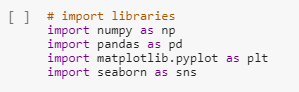
\includegraphics[width=9cm]{IMG/2.png} 
\end{center}

Importamos el archivo


\begin{center}
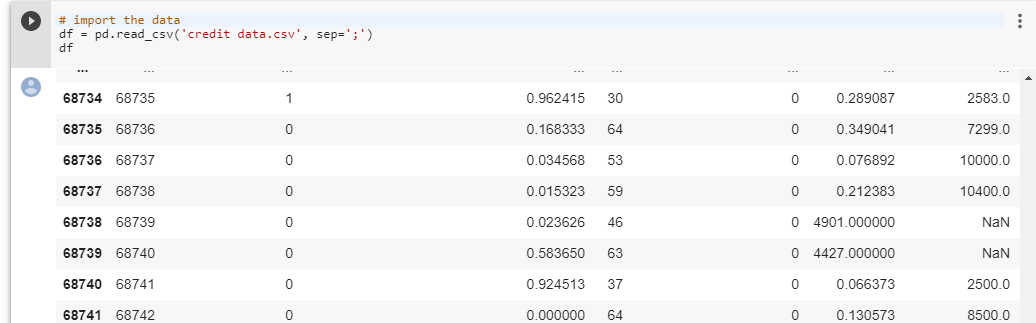
\includegraphics[width=9cm]{IMG/3.png} 
\end{center}

revisamos los tipos

\begin{center}
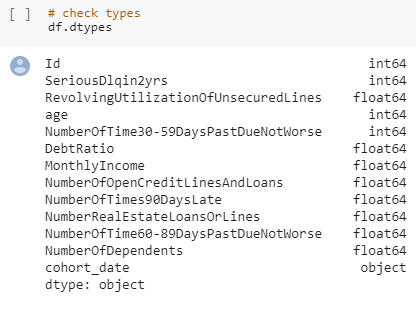
\includegraphics[width=9cm]{IMG/4.png} 
\end{center}


verifica que las fechas est\'en bien cargadas

\begin{center}
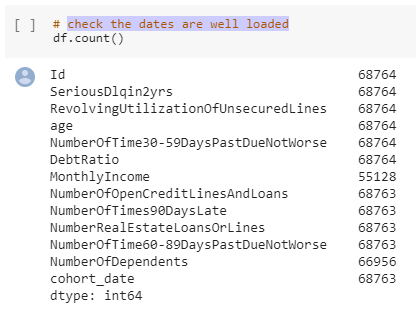
\includegraphics[width=9cm]{IMG/5.png} 
\end{center}


- Imputaci\'on de valores faltantes.

\begin{center}
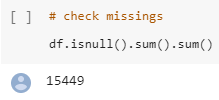
\includegraphics[width=5cm]{IMG/6.png} 
\end{center}

\begin{center}
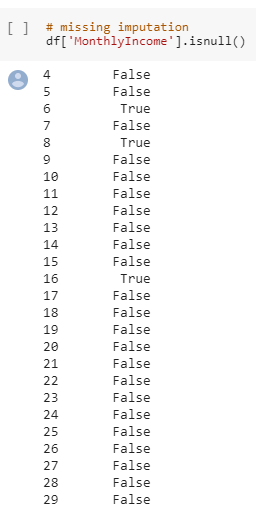
\includegraphics[width=5cm]{IMG/7.png} 
\end{center}

- Seleccione la muestra de datos para el informe

\begin{center}
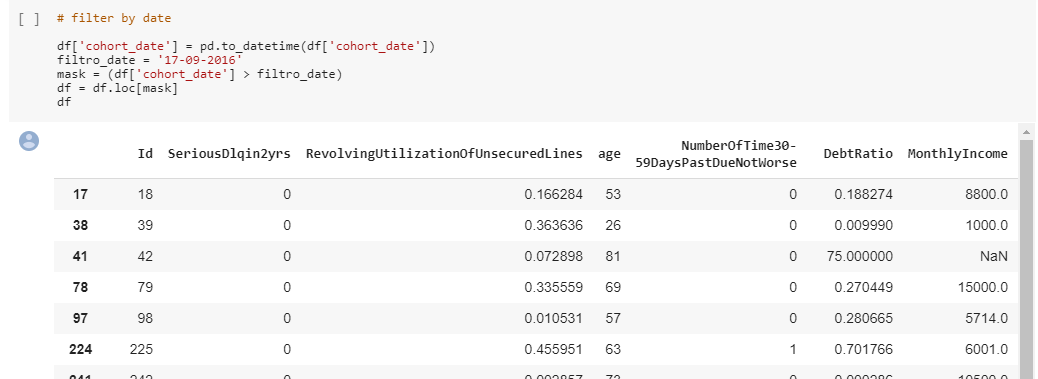
\includegraphics[width=15cm]{IMG/8.png} 
\end{center}

- Crear variables intermedias

\begin{center}
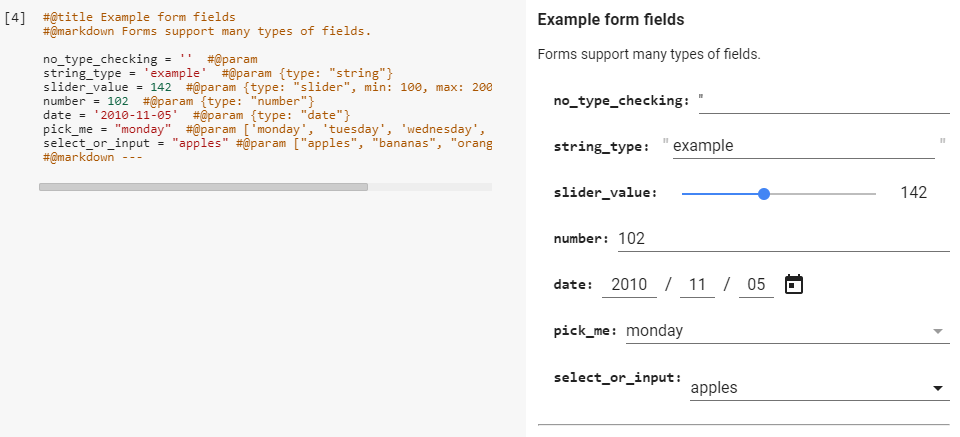
\includegraphics[width=15cm]{IMG/9.png} 
\end{center}

- Creaci\'on de Reportes

Reporte por a\~no

\begin{center}
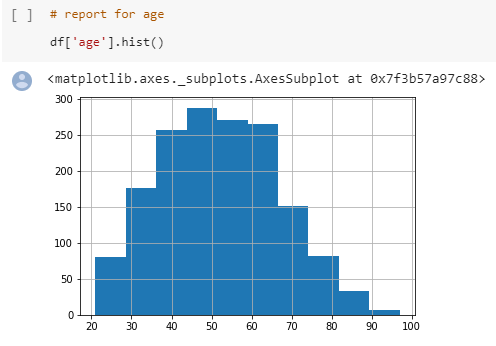
\includegraphics[width=9cm]{IMG/10.png} 
\end{center}

Reporte por mes

\begin{center}
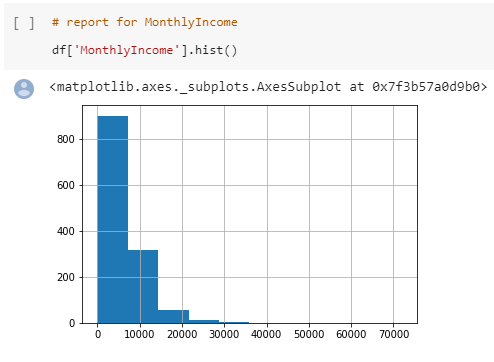
\includegraphics[width=9cm]{IMG/11.png} 
\end{center}

\section{Conclusiones} 

-	Como conclusi\'on tenemos que Colab es muy convenientes para principiantes que quieran experimentar con machine learning y  sin incurrir en costos de procesamiento cloud. Adem\'as, el ambiente de trabajo ya viene con muchas librer\'ias instaladas listas para utilizar.

\end{document}

